\documentclass{standalone}

\usepackage[utf8]{inputenc}
\usepackage{default}
\usepackage{amsfonts} % if you want blackboard bold symbols e.g. for real numbers
\usepackage{graphicx} % if you want to include jpeg or pdf pictures
\usepackage{lmodern}
\usepackage{amsmath}
\usepackage{amssymb}
\usepackage{algorithmic}
\usepackage{algorithm}


\usepackage{pgfplots}
\usepackage{filecontents}
\begin{document}

%\caption{LOG elapsed time for N agents\label{time}}
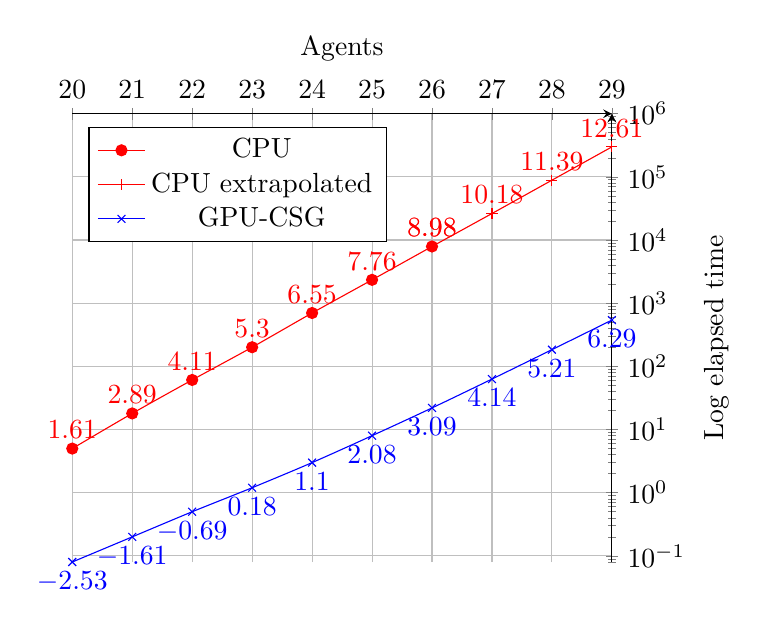
\begin{tikzpicture}[align=left]
\begin{axis}[
  xmin = 20,
  xmax = 29,
  ymax = 10e5,
  grid,
  xlabel={Agents},
  ylabel={Log elapsed time},
  xtick={20,...,29},
  axis lines=right, 
  legend pos= north west,
  ymode=log
    ]
\addplot[ mark = *,red,smooth,nodes near coords] coordinates  
{( 20, 5 )
 ( 21, 18 )
 ( 22, 61 )
 ( 23, 201 )
 ( 24, 700 )
 ( 25, 2344 )
 ( 26, 7910 )
 }; 
 \addplot[ mark = +,red,smooth,nodes near coords] coordinates  
{
 ( 26, 7910 )
 ( 27, 26302 )
 ( 28, 88644)
 ( 29, 298267)
 }; 
 
 \addplot[ mark = x,blue,smooth,nodes near coords,nodes near coords align={below}] coordinates  
{( 20, 0.08 )
 ( 21, 0.2 )
 ( 22, 0.5 )
 ( 23, 1.2 )
 ( 24, 3 )
 ( 25, 8 )
 ( 26, 22 )
 ( 27, 63 )
 ( 28, 184)
 ( 29, 541)
 }; 

\legend{CPU,CPU extrapolated,GPU-CSG}

\end{axis}
\end{tikzpicture}

\end{document}
